%%%% Paramétrage du cours %%%%
\def\xxactivite{Cours}

\fichefalse \proftrue \tdfalse \courstrue

\def\xxnumchapitre{Chapitre 2 \vspace{.2cm}}
\def\xxchapitre{\hspace{.12cm} Représentation des nombres en mémoire}

\def\xxcompetences{%
\textsl{%
\textbf{Savoirs et compétences :}\\
\begin{itemize}[label=\ding{112},font=\color{bleuxp}] 
\item Représentation des entiers positifs sur des mots de taille fixe.
\item Représentation des entiers signés sur des mots de taille fixe.
\item Entiers multi-précision de Python.
\item Distinction entre nombres réels, décimaux et flottants.
\item Représentation entre nombres réels, décimaux et flottants.
\item Représentation des flottants sur des mots de taille fixe. Notion de mantisse, d'exposant. 
\item Précision des calculs en flottants.
\end{itemize}
}}

\def\xxfigures{
%\includegraphics[width=\linewidth]{matlab}
%\\
%\textit{Modèle du pilote hydraulique avec pilotage interactif.}
}%figues de la page de garde

\input{\repRel/Style/pagegarde_cours_minitoc}
\setlength{\columnseprule}{.1pt}

\vspace{2cm}
\pagestyle{fancy}
\thispagestyle{plain}

%%%%%%%%%%%%%%%%%%%%%%%

\section{Bases de numération}

Le système de numération courant est le système décimal (ou base 10). 
On décompose un entier en dizaines, centaines, milliers, etc. 
L'essentiel est alors qu'il y ait strictement moins de dix éléments dans chaque type de paquet. Ce nombre d'éléments peut être représenté par un chiffre.
On écrit alors tous les chiffres à la suite. À gauche, on place les \textbf{chiffres de poids fort} (\textit{most significant digit}). À droite, les \textbf{chiffres de poids faible}  (\textit{least significant digit}).

Ainsi $2735$ représente deux milliers plus sept centaines plus trois dizaines plus cinq unités.

\begin{defi}{Ecriture d'un nombre dans une base }
De manière générale :%, avec $B=10$ et $n\in\N$,
$$\displaystyle\underline{a_{n}a_{n-1}\ldots a_{1}a_{0}}_{~B} =
\sum_{k=0}^{n}a_{k}B^{k},~ \textrm{ et }~\forall k \in \iif{0;n},~ a_k\in\ii{0;B}.$$ 
On note $B$ la base, $a_k$ le chiffre de rang $k$.
\end{defi}

\begin{exemple}
Décomposition de 247 en base 10 : $247_{(10)} = 2\cdot 10^2 + 4\cdot 10^1 + 7\cdot 10^0$.

Décomposition de $1001_2$ en base 2 : $1001_2 = 1\cdot 2^{11_2} + 0\cdot 2^{10_2} + 0\cdot 2^{1_2} + 1\cdot 2^{0_2} 
= 1\cdot 2^{3_{10}} + 0\cdot 2^{2_{10}} + 0\cdot 2^{1_{10}} + 1\cdot 2^{0_{10}}$.
\end{exemple}



\subsection{Les systèmes de numération}
\subsubsection{Système décimal}
Le système décimal est le système universellement utilisé. C'est la base de référence, ce qui signifie qu'un nombre est de manière implicite écrite en décimal, dès lors qu'il est écrit sans précision de base. 

En python, les chiffres sont \textbf{affichés} par défaut dans le système décimal. 

\subsubsection{Système binaire}

C'est la base de numération couramment utilisée en électronique ou informatique. C'est un système en base 2, l'écriture des nombres est donc composée des caractères de 0 et 1. 

\begin{exemple}~\\

\begin{minipage}[c]{.4\linewidth}
En binaire on compte de la manière suivante : 
\begin{center}
\begin{tabular}{|c|c|}
\hline
Base 10 & Base 2 \\
\hline \hline
0 & 0000 \\ \hline
1 & 0001 \\ \hline
2 & 0010 \\ \hline
3 & 0011 \\ \hline
4 & 0100 \\ \hline
\end{tabular}
\end{center}
\end{minipage} \hfill
\begin{minipage}{.57\linewidth}
\textit{Convertir $\left(11011001\right)_2$ en base 10.}

\textit{Convertir $\left(42\right)_{10}$ en base 2.}
\end{minipage}
\end{exemple}

En Python, il est possible de manipuler des nombres en binaires en utilisant le préfixe \texttt{0b}. Ainsi, \texttt{0b111} est interprété comme l'entier 7. 
Il est aussi possible de convertir des entiers en binaires avec la fonction bin. Le résultat est une chaîne de caractère (\texttt{str}) de la forme \texttt{'0b111'}.

\subsubsection{Système hexadécimal}
Ce système à base 16 est le plus utilisé en électronique numérique car il permet une représentation compacte ce qui, dans les systèmes actuels à grande capacité mémoire, est un avantage non négligeable. 
Ainsi, les chiffres de ce système de numération sont 0, 1, 2, 3, 4, 5, 6, 7, 8, 9, A, B, C, D, E, F.  

\begin{exemple} ~\\
\begin{minipage}[c]{.6\linewidth}
En hexadécimal on compte de la manière suivante : 
\begin{center}
\begin{tabular}{|c|c|c||c|c|c|}
\hline
Base 10 & Base 2 & Base 16 & Base 2 & Base 10 & Base 16 \\
\hline \hline
0 & 0000 & 00 & 10 & 1010 & 0A \\ \hline
1 & 0001& 01 & 11  & 1011 & 0B \\ \hline
2 & 0010& 02 & 12  & 1100 & 0C \\ \hline
3 & 0011& 03 & 13  & 1101 & 0D \\ \hline
4 & 0100& 04 & 14  & 1110 & 0E \\ \hline
5 & 0101& 05 & 15  & 1111 & 0F \\ \hline
6 & 0110& 06 & 16  & 1 0000 & 10\\ \hline
7 & 0111& 07 & 17  & 1 0001 & 11 \\ \hline
8 & 1000& 08 & 18  & 1 0010 & 12 \\ \hline
9 & 1001& 09 & 19  & 1 0011 & 13 \\ \hline
\end{tabular}
\end{center}
\end{minipage}% \hfill
\begin{minipage}[t]{.37\linewidth}
Convertir $\left(BC5 \right)_{16}$ en base 10.

Convertir $192$ en base 16.
\end{minipage}
\end{exemple}


En Python, il est possible de manipuler des nombres en hexadécimal en utilisant le préfixe \texttt{0x}. Ainsi, \texttt{0xA1} est interprété comme l'entier 162. 
Il est aussi possible de convertir des entiers en hexadécimal avec la fonction \texttt{hex}. Le résultat est une chaîne de caractère (\texttt{str}) de la forme \texttt{'0xa1'}.


\subsection{Algorithme de décomposition d'un entier dans une base}
\begin{methode}
La méthode générale pour décomposer un entier $n$ en base $k$ est la suivante :
\begin{itemize}
\item on effectue des divisions euclidiennes successives par k jusqu’à avoir un quotient nul ;
\item on récupère les restes en remontant les calculs.
\end{itemize}
\end{methode}

\begin{lstlisting}
def decomposition(x:int, k:int)->str:
    """Donne la décomposition de l'entier x dans la base k.
    Entrées :
        x(int) : le nombre entier à écrire dans une nouvelle base
        k(int) la base de décomposition
    Sortie :
        le nombre dans la nouvelle base sous forme de chaine de caractères
    """
    n = x
    chaine = ''
    if n==0:
        chaine='0'
    while n > 0:
        r = n % k
        chaine = str(r) + chaine
        n = n // k
    return(chaine)
\end{lstlisting}

\section{Représentation des entiers sur un ordinateur}
\subsection{Cadre}
\begin{defi}{Mot-machine}
En architecture informatique, un mot est une unité de base manipulée par un microprocesseur. On parle aussi de mot machine. La taille d’un mot s’exprime en bits. Elle est souvent utilisée pour classer les microprocesseurs (32 bits, 64 bits, etc.).
\end{defi}

Sur un ordinateur on travaille sur des mots-machine de 64 bits (8 octets).

Les opérations d’addition et de multiplication d’entiers internes au processeur se font sur 64 bits.
De manière générale, on s’intéressera au fonctionnement sur des ordinateurs travaillant sur des mots de $n$ bits
($n \geq 2$).


Par ailleurs, sur les disques durs, les donées sont stockées sous forme binaire. Ainsi, 
un octet = \SI{8}{bits}, un kilo octet~= \SI{1000}{octet} \textit{etc}.


\subsection{Représentation des entiers}
Les entiers sont directement codés en binaire. Lorsque les mots-machines sont codés sur $n$ bits, il est alors possible de coder des nombres compris entre 0 et $2^n-1$.
\begin{rem}
\begin{itemize}
\item On peut alors observer des dépassements de capacité : si les mots sont codés sur 4 bits, $(1100)_2 + (1000)_2 = (0100)_2$ (et non $(10100)_2$). Dans ce cas, la retenue est perdue. 
\item En Pyton, les entiers ne sont pas codés sur un nombre de bits défini. On est seulement limité par la mémoire de la machine.
\end{itemize}
\end{rem}
\subsection{Représentation des entiers relatifs -- Complément à 2}

Lorsque les mots sont codés sur $n$ bits et qu'on souhaite coder des entiers positifs et négatifs, on pourra coder des nombres compris dans l'intervalle $\llbracket-2^{n-1},2^{n-1}-1\rrbracket$. Les nombres positifs seront codés en binaire comme vu précédemment. 

Les nombres négatifs seront codés selon la méthode du complément à 2. 
\begin{methode}
Si les mots sont codés sur $n$ bits, si on souhaite coder $a<0$, $a$ sera codé comme l'entier naturel $a+2^n$. 
\end{methode}

\begin{exemple} 
\begin{multicols}{2}
Soit un système où les entiers relatifs sont codés sur 3 bits. On peut donc coder des nombres compris dans $\llbracket-4,3\rrbracket$.
\begin{itemize}
\item 2 est codé par $2=(010)_2$;
\item $-2$ est codé par $-2+2^3 = 6 = (110)_2$.
\end{itemize}  
\textit{Remarques :}
\begin{itemize}
\item les nombres négatifs commencent donc par $1$;
\item pour convertir $a=(110)_2$ en base 10 lorsque le codage est sur 3 bits, on a :$a= (110)_2 - 2^3 = 6 - 8 = -2$.
\end{itemize}  
\end{multicols}
\end{exemple}

\section{Représentation des nombres réels}
\subsection{Conversion de la partie fractionnaire des nombres réels}

En notation décimale, les chiffres à gauche de la virgule représentent des entiers, des dizaines, des centaines, etc. et ceux à droite de la virgule, des dizièmes, des centièmes, des millièmes, etc.


\begin{exemple}
$$
3,3125_{ (10)}	=	3\cdot 10^0 + 3\cdot10^{- 1} + 1\cdot10^{- 2} + 2\cdot10^{ -3} + 5\cdot10^{ -4}
$$
\end{exemple}

Par analogie, pour écrire un nombre binaire à virgule, on utilise les puissances négatives de 2.

\begin{exemple}
\begin{eqnarray*}
11,0101_{(2)} &=&	1\cdot 2^{1} + 1\cdot 2^{0} + 0\cdot 2^{-1} + 1\cdot 2^{- 2} + 0\cdot 2^{-3} + 1\cdot 2^{- 4}\\
		 &=&    2   +   1   +    0    +   0,25  +     0     +   0,0625\\
		 &=&   3,3125_{(10)}\\
\end{eqnarray*}
\vspace{-1cm}
\end{exemple}


Le codage de la partie entière (3 dans l’exemple précédent) ne pose pas de problèmes particuliers. Pour la partie fractionnaire (0,3125), il est nécessaire d’adapter la procédure.

\begin{methode}
\textbf{Conversion d'une partie fractionnaire en binaire}

\begin{enumerate}
\item On multiplie la partie fractionnaire par 2. 
\item La partie entière obtenue représente le poids binaire (limité aux seules valeurs 0 ou 1). 
\item La partie fractionnaire restante est à nouveau multipliée par 2.
\item On procède ainsi de suite jusqu’à ce qu’il n’y ait plus de partie fractionnaire ou que le nombre de bits obtenus correspond à la taille du mot mémoire dans lequel on stocke cette partie.
\end{enumerate}
\end{methode}


\begin{exemple}
\textit{Conversion de la partie fractionnaire 0,3125}

\begin{center}
\begin{tabular}{cccccc|c|cc}
\cline{7-7}
0,3125 & x & 2 & = & 0,625 & = & 0 & + & 0,625 \\
0,6250 & x & 2 & = & 1,250 & = & 1 & + & 0,250 \\
0,2500 & x & 2 & = & 0,500 & = & 0 & + & 0,500 \\
0,5000 & x & 2 & = & 1,000 & = & 1 & + & 0,000 \\
\cline{7-7}
\end{tabular}
\end{center}
On considère les parties entières de haut en bas :
$0,3125_{(10)}=0,0101_{(2)}$.
%\begin{center}
%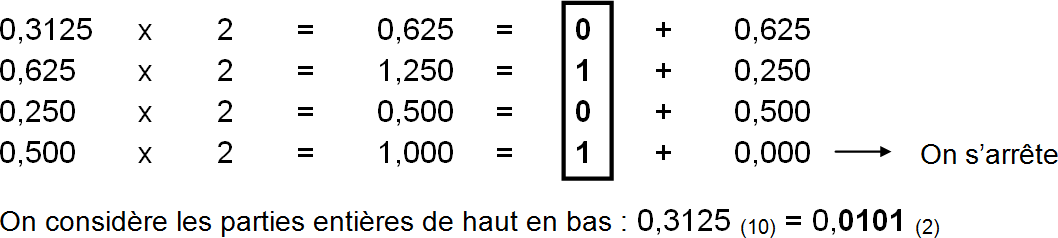
\includegraphics[width=.7\textwidth]{images/reel_0}
%\end{center}
\end{exemple}

%\begin{rem}
%\textbf{Inconvénients}
%
%Savoir coder la partie fractionnaire d’un nombre à virgule ne suffit pas pour coder tous les nombres à virgule en binaire. En effet, la gestion d’une virgule virtuelle par programme n’est pas aisée. De plus, cette méthode ne permet pas de représenter des nombres très grands ou très petits comme le nombre d’Avogadro ($6,02214129.. \cdot  10^{23}$) ou la constante de Planck ($6,62606957 \cdot 10^{- 34}$).
%\end{rem}

\begin{exemple}
\textit{Convertir la partie fractionnaire 0,1}
\end{exemple}
